\documentclass[10pt,conference]{IEEEtran}
\usepackage{cite}
\usepackage{amsmath,amssymb,amsfonts}
\usepackage{graphicx}
\usepackage{float}
\usepackage{placeins}
\usepackage{booktabs}
\usepackage{tabularx}
\usepackage{textcomp}
\usepackage{pifont}
\usepackage{xcolor}
\usepackage[hyphens]{url}
\usepackage{fancyhdr}
\usepackage{hyperref}

% Keep figures close to the paragraph that introduces them.
\setlength{\intextsep}{6pt plus 1pt minus 1pt}
\setlength{\textfloatsep}{7pt plus 1pt minus 2pt}
\setlength{\floatsep}{6pt plus 1pt minus 1pt}
\setlength{\abovecaptionskip}{3pt}
\setlength{\belowcaptionskip}{0pt}

% Ensure letter paper.
\pdfpagewidth=8.5in
\pdfpageheight=11in

\newcommand{\hpcayear}{2027}
\newcommand{\hpcasubmissionnumber}{NaN}
\title{CuPath: Cuckoo-Filter-Guided Memory Request Transformation for Wafer-Scale GPUs}

% Camera-ready fields. Keep the camera-ready switch disabled for submission.
%\def\hpcacameraready{}
\newcommand{\hpcapubid}{0000--0000/00\$00.00}
\newcommand\hpcaauthors{First Author and Second Author}
\newcommand\hpcaaffiliation{Affiliation}
\newcommand\hpcaemail{Email(s)}

\input{hpca-template}

%%%%%%%%%%%%%%%%%%%%%%%%%%%%%%%%%%%%%%%%
%%%%%%%% -- PAPER CONTENT STARTS -- %%%%

\begin{abstract}
Wafer-scale GPUs expose distributed compute and HBM as one logical device, yet
a cache-line miss may traverse the requesting GPM's L2 and RDMA endpoint, the
wafer network, and the home GPM's RDMA endpoint, L2, and HBM.  Existing designs
optimize each component using only locally visible state.  We show that useful
request state changes during a request lifetime: real accesses expose a predictive relation,
L2 state eliminates already resident or pending work, requesting-GPM RDMA exposes
cross-L1 and destination aggregation, and returned data exposes reuse.  We
propose \emph{CuPath}, which connects these decisions through a common bounded
real-demand predictor design and one typed Cuckoo Filter per L2 slice.  CuPath
first filters a directly adjacent local candidate and, when useful, exposes it
with the triggering miss through a paired HBM access,
then uses Filter-maintained pending-line and active-batch state to merge remote
requests and permits a remote candidate only to piggyback an existing
home-GPM/page batch, and finally retains useful
returned data in the existing requesting-GPM L2 while feeding outcomes back to
prediction metadata.  Exact tags, MSHRs, and transaction tables remain
authoritative; unavailable speculative opportunities are dropped immediately.
CuPath adds no global scheduler or new cache level.
We evaluate both end-to-end performance and the cache, DRAM, RDMA, packet, and
wafer-traversal work removed at each boundary.
\end{abstract}

\section{Introduction}
\label{sec:introduction}

Wafer-scale GPUs are emerging as a practical way to continue GPU scaling
beyond the size, yield, and manufacturability limits of a monolithic die.
MCM-GPUs first address the monolithic-die limits by connecting multiple GPU
processing modules (GPMs) through silicon interposers, expanding compute
resources and memory capacity within a package
\cite{arunkumar2017mcm,mi350}.  Wafer-scale integration extends the
multi-module organization across an entire wafer.  Many GPMs and
distributed HBM stacks are connected by a high-bandwidth, low-latency
on-wafer network and exposed as one logical GPU
\cite{pal2019architecting,hu2024wafer,xu2025exploring}.  Wafer-scale
integration is approaching commercial reality, with TSMC's System-on-Wafer
technology planned for 2027 \cite{TSMCAdvancedPackaging}.  However, placing
more resources on one wafer does not make every memory access local.

The on-wafer mesh provides high-bandwidth communication between GPMs, but each
physical page still resides in the HBM of one home GPM.  A local L1 miss
reaches the address-selected L2 slice and, on an L2 miss, accesses local HBM.
The returned cacheline fills the local cache hierarchy before reaching the
requesting CU.

A remote L1 miss is routed through the requesting GPM's RDMA endpoint, the
on-wafer network, and the home GPM's RDMA endpoint and L2 before reaching the
home-GPM HBM when necessary.  The response returns across the wafer to the
requesting GPM's L1, and the baseline does not retain remote returns in the
requesting GPM's L2.  Duplicate or repeated accesses can therefore
pay endpoint, network, cache, and memory costs multiple times.  Prior
multi-GPU studies show that remote-access cost and sharing behavior vary widely
across applications \cite{khairy2020locality,zhang2023characterizing}.

Local memory exposes a mismatch between regular GPU access patterns and
cacheline-by-cacheline processing.  Half of the workloads have L2 read miss
rates above 80\%, allowing related adjacent demands to reach HBM as separate
memory requests.  Fetching every adjacent line is unsafe because the candidate
may already be resident, already be pending, or never be requested.  Local
acceleration therefore requires a selective decision that learns a recurring
relation from real demands and checks current L2 state before adding another
cacheline to the HBM access and L2 fill path.

Remote memory remains expensive even with a low-latency on-wafer network.  A
remote miss still consumes requesting-GPM RDMA service, network bandwidth,
home-GPM RDMA service, and home-GPM cache or HBM resources before the response
returns.  Finite RDMA width and outstanding capacity further make related
requests contend for the same endpoint resources.  Overall, 42.8\% of sampled
remote reads expose either an in-flight duplicate or a nearby same-page
partner.  The baseline then places returned data only in a private
requesting-GPM L1, so an access from another CU or after L1 eviction repeats
the remote path.  Later touches account for 33.6\% of remote reads, but
retaining every return in the requesting GPM's L2 would waste capacity on
one-touch data \cite{zhao2020selective,zhang2023sac}.  Remote acceleration must
therefore aggregate requests before network injection and retain returned data
in the existing requesting-GPM L2 only after reuse is observed.

We propose \emph{CuPath}, which uses a lightweight demand predictor and one
typed Cuckoo Filter per L2 slice to identify and optimize memory requests
during memory-path traversal \cite{fan2014cuckoo}.  The predictor proposes
at most one adjacent candidate from real demand history.  The Filter records
compact pattern, residency, in-flight, and reuse state, allowing later
stages to quickly reject work that is already present or unlikely to help.
The Filter is a control structure rather than a data cache.  Exact tags,
MSHRs, and RDMA transaction tables remain authoritative.

CuPath applies the recorded state in three places.  First, the
local L2 removes resident or pending candidates and, when the remaining sibling is
compatible with the demand, exposes both adjacent cachelines through one paired
HBM access.  Second, requesting-GPM RDMA uses
\textsc{Remote-Pending} to identify possible duplicate lines and
\textsc{Remote-Batch} to locate a joinable home-GPM/page batch. Exact RDMA
tables confirm the Filter results before merging identical requests or grouping
different lines into one packet;
a predicted remote line is allowed only when a free position exists in
an existing batch.  Third, after the response returns, CuPath uses real reuse
evidence to retain useful remote data in the existing requesting-GPM L2, avoiding a
later wafer traversal.  Outcomes feed back to the predictor so that useful
relations remain active and unused ones are suppressed.

CuPath is deliberately work-conserving.  CuPath never delays a demand while
waiting for a partner, never creates a remote packet for a predicted line, and
immediately falls back to the original path when metadata or downstream
resources are unavailable.  CuPath adds no global scheduler or new cache
level.  Figure~\ref{fig:cupath-overview} summarizes how a request
is filtered, combined with useful in-flight work, and selectively retained
during memory-path traversal.

\begin{figure}[t]
  \centering
  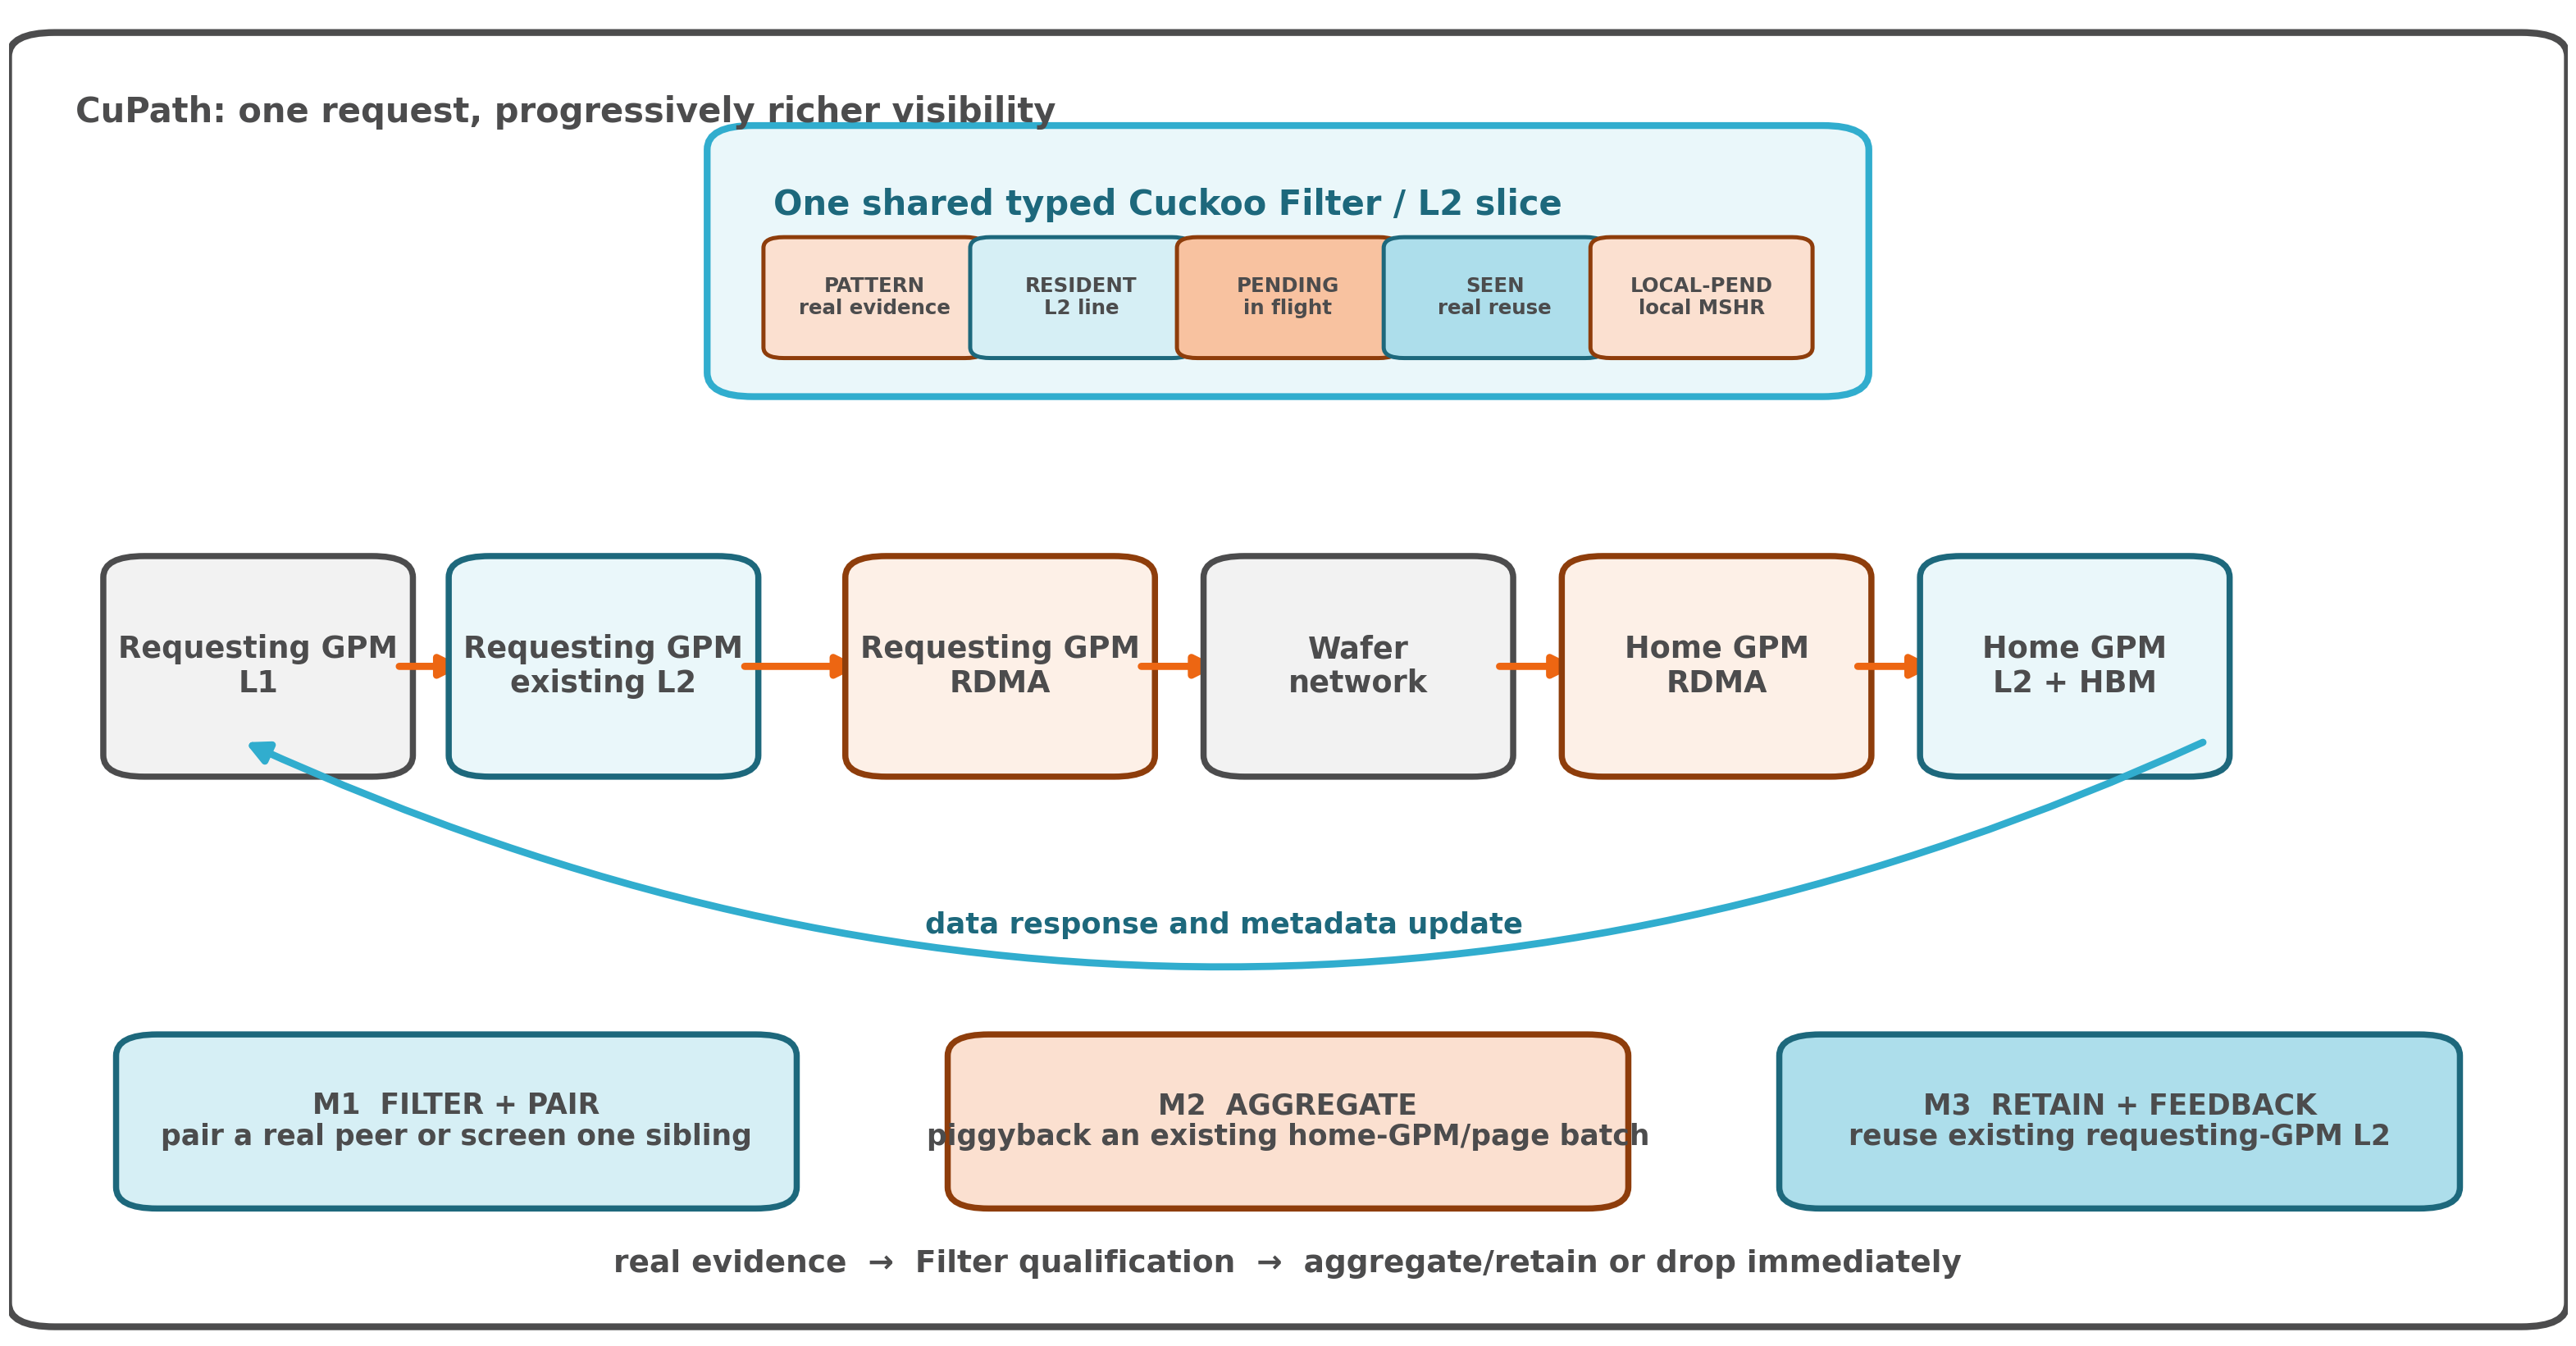
\includegraphics[width=\columnwidth]{Figure/CuPathoverall.png}
  \caption{CuPath continuously filters a predicted request, aggregates the
  request only with compatible in-flight work, and retains returned data in the existing
  requesting-GPM L2.}
  \label{fig:cupath-overview}
\end{figure}

Across fourteen GPU workloads, CuPath improves every workload and achieves a
1.534$\times$ geometric-mean speedup.  More importantly, the speedup follows
from work removed along the path.  CuPath reduces L2 tag lookups by 22.6\%,
on-wafer packets by 48.2\%, and repeated wafer traversals by 30.8\%.

We make the following contributions.

\begin{itemize}
  \item We identify and quantify how predictive locality, cache state, remote
  aggregation, and reuse become visible at different points in a wafer-scale
  memory-request lifetime.

  \item We propose CuPath, an end-to-end memory-path design that couples a
  bounded real-demand predictor and per-slice typed Cuckoo Filter with the
  existing HBM controller, RDMA engine, and requesting-GPM L2.

  \item We implement and evaluate CuPath without adding a global scheduler,
  cache level, achieving a 1.534$\times$
  geometric-mean speedup while substantially reducing cache and network work.
\end{itemize}

\section{Background}
\label{sec:background}

\subsection{Cuckoo Filters}
\label{sec:background-cuckoo}

A Cuckoo Filter is an array of buckets, where each bucket contains several
slots that are read together \cite{fan2014cuckoo}.  Each occupied slot stores a
short fingerprint rather than a complete key.  Hashing a key produces its
fingerprint and two possible bucket locations.  A lookup checks both buckets,
while an insertion places the fingerprint in an empty slot or relocates an
existing fingerprint when both buckets are full.  The structure also supports
deletion.  A negative lookup proves absence, while a positive lookup remains a
possible match and must be checked against exact state.

For example, suppose the address of a cacheline produces fingerprint $f$ and
maps to buckets 3 and 11.  When the cacheline is filled into L2, the filter
stores $f$ in one of the four slots in either bucket.  A later L2 data request
recomputes the same fingerprint and bucket locations.  If neither bucket
contains $f$, the cacheline is not resident and the request can skip the L2 tag
and data array lookup before continuing along the miss path.  If either bucket
contains $f$, the request checks the exact L2 tag.  A tag hit reads the data
array, while a false positive simply follows the normal cache miss path.  The
fingerprint is deleted when the cacheline is evicted.  If an insertion fails,
the filter conservatively sends later requests to the exact L2 lookup.  The
filter therefore avoids unnecessary cache probes without changing correctness
\cite{moshovos2001jetty}.  It stores only metadata and has finite lookup and
update bandwidth.

\subsection{RDMA Request Processing}
\label{sec:background-rdma}

RDMA moves data between GPMs without involving a host processor in each
transfer \cite{kalia2016design,wei2018deconstructing,mittal2018revisiting}.
Each GPM's RDMA endpoint connects both the private L1 caches and the shared L2
to the wafer mesh.  The L1 facing path contains a request table and a pair of
TX and RX interfaces.  The request table retains every remote memory
transaction issued by local L1 caches until its response returns.  TX sends
these requests to remote GPMs, while RX returns incoming responses to the
corresponding L1 requests.  The L2 facing path provides another pair of TX and
RX interfaces.  RX forwards incoming remote requests to the local L2, and TX
sends the resulting data responses back to their requesting GPMs.  A bounded
request table limits the number of requester transactions in flight and
propagates backpressure to L1 when no entry is available.

Figure~\ref{fig:baseline-overview} follows a baseline remote request from the
requesting GPM's L1 to the owner GPM's L2.  At \ding{192}, address translation
identifies a remote page, and the L1 miss allocates a request table entry before
reaching TX.  At \ding{193}, requester TX injects the request packet into the
wafer mesh.  At \ding{194}, the owner L2 facing RX accepts the packet.  At
\ding{195}, RX forwards the recovered cacheline request to the owner L2.  An
owner L2 hit supplies the data directly, while an L2 miss accesses owner HBM.
The response returns through owner TX, the wafer mesh, and requester RX.  The
request table then completes the stored transaction and delivers the data to
the original L1 request.  In the baseline, same line misses from different
private L1 caches allocate separate entries and network packets before the
owner L2 can observe and merge them.

\subsection{HBM Organization and Row Locality}
\label{sec:background-hbm}

HBM provides high bandwidth through a wide interface and many independently
operated banks \cite{li2016exploring,wang2022shuhai,micron_hbm2e}, but each
bank still follows the conventional DRAM row buffer model
\cite{rixner2000memory,ding2013reshaping}.  A physical address is decomposed
into channel, rank, bank group, bank,
row, and column fields.  An activate command copies one row into the bank row
buffer.  A following column read to that open row can transfer data without
another activation.  A request to a different row must first precharge the
bank and then activate the new row.  Serving several nearby columns while a row
remains open can therefore avoid repeated precharge and activation latency
\cite{rixner2000memory}.  HBM address mapping and the order in which requests
reach the controller determine whether this locality is visible
\cite{li2016exploring,wang2022shuhai,wang2019mac}.  The simulator models these
effects explicitly with transaction and command queues, bank state, burst
timing, and separate activate, column, and precharge commands.  Its ordinary
close page path attaches an automatic precharge to a completed access.  When
two linked adjacent requests are simultaneously ready and map to the same
physical bank and row, the controller changes the first operation into a read
without automatic precharge, keeps the row open, and issues the adjacent column
next.  The row is not retained when the second request is unavailable, maps to
a different row, or would bypass an older conflicting request.  Adjacent line
selection is therefore useful because it creates a bounded opportunity for
row reuse, while the controller remains responsible for validating the actual
HBM mapping and timing constraints.


\section{Observations: Information Revealed Along the Memory Path}
\label{sec:observations}

We use the same 14 workloads as the evaluation to examine when a request
reveals information that can remove or combine memory-system work. O1
establishes the end-to-end cost. O2 and O3 motivate local paired HBM access,
O4 and O5 motivate requester-side remote aggregation, and O6 motivates
selective reuse in the existing requesting-GPM L2.

\noindent\textbf{O1: Cost of a Full Memory Path.}
We measure each component from request arrival until it forwards the request
or response, charge local communication to the receiving component, and group
RDMA processing and wafer traversal as Remote Communication. We count only
completed demand-read MSHR leaders and exclude L1 and L2 MSHR waiting. As
Fig.~\ref{fig:obs-full-path} shows, an HBM-reaching local path takes
74--563~ns, while the seven workloads with a qualifying remote demand path
take 0.45--7.19~$\mu$s. The local L2 demand-read miss rate ranges from 2.8\%
to 100\%, and the dominant latency component changes across workloads. The
bottleneck is therefore an end-to-end path property rather than the property
of one fixed cache, network, or memory component.

\begin{figure}[!t]
  \centering
  \includegraphics[width=\columnwidth]{../../akkalat/results/2026-07-22-baseline-complete-observation/observation-analysis/figures/o1_memory_path_latency.pdf}
  \caption{Normalized full-path latency and local-L2 demand-read miss rate for
  local (L) and remote (R) MSHR leaders. MSHR waiting is excluded, and
  ``--'' denotes no qualifying remote demand path.}
  \label{fig:obs-full-path}
\end{figure}

\noindent\textbf{O2: Local Misses Expose Adjacent Demand Pairs.}
We record each real L2 read miss and locate the nearest earlier miss to the
adjacent cacheline in the same aligned access region. Within 16 L2 cycles,
13 of 14 workloads expose such a relation for 5.0\%--50.0\% of their misses.
Weighted across all workloads, adjacent relations cover 7.3\%, 15.0\%,
22.0\%, and 33.0\% of misses within 0, 4, 16, and 64 cycles, respectively
(Fig.~\ref{fig:obs-adjacent-window}). KMeans exposes no relation in the
measured window, showing why adjacent access should be learned from real
demands rather than generated unconditionally.

\begin{figure}[!t]
  \centering
  \includegraphics[width=\columnwidth]{../../akkalat/results/2026-07-22-baseline-complete-observation/observation-analysis/figures/o2_adjacent_line_cdf.pdf}
  \caption{Fraction of real L2 read misses whose adjacent cacheline miss
  arrived within a short preceding window.}
  \label{fig:obs-adjacent-window}
\end{figure}

\noindent\textbf{O3: Physical Mapping Makes Adjacent Work HBM-Friendly.}
We apply the controller's bank, row, column, and aligned-access mapping to
physical read arrivals. Within 16 controller cycles, 29.1\% of reads find an
earlier read in the same aligned HBM access unit, while only 6.2\% find a
different column in the same row (Fig.~\ref{fig:obs-dram-locality}). Thus,
the strongest local relation is not arbitrary spatial proximity but the
specific adjacent-line relation already aligned with the controller's access
unit. M1 learns this relation from completed demand pairs and attempts a
paired access only after exact cache and pending state remove an already
available half. Otherwise, the original singleton request proceeds.

\begin{figure}[!t]
  \centering
  \includegraphics[width=\columnwidth]{../../akkalat/results/2026-07-22-baseline-complete-observation/observation-analysis/figures/o3_dram_physical_locality.pdf}
  \caption{CDF of physical-read proximity for an aligned HBM access unit,
  same-row accesses, row changes within a bank, and different-bank accesses.}
  \label{fig:obs-dram-locality}
\end{figure}

\noindent\textbf{O4: Remote Requests Amplify Work Before Owner Coalescing.}
Across ten workloads, 713,568 sampled remote operations traverse requester
RDMA, the wafer network, and owner-GPM RDMA before any owner-L2 MSHR can merge
their memory work. One logical byte produces 6.05 network byte-hops, and mean
remote-transaction latency ranges from 0.465 to 7.787~$\mu$s
(Fig.~\ref{fig:obs-remote-amplification}). An owner-L2 MSHR may still reduce
later HBM accesses, but it acts only after requester endpoint and forward
network work has already been paid. Removing redundancy at requesting-GPM
RDMA therefore eliminates work that owner-side coalescing cannot recover.

\begin{figure}[!t]
  \centering
  \includegraphics[width=\columnwidth]{../../akkalat/results/2026-07-22-baseline-complete-observation/observation-analysis/figures/o4_remote_amplification.pdf}
  \caption{Network byte-hops per logical remote byte and mean end-to-end
  remote-operation latency. ``--'' denotes no remote operation in the O4
  trace window.}
  \label{fig:obs-remote-amplification}
\end{figure}

\noindent\textbf{O5: Requester RDMA Reveals Two Aggregation Scopes.}
Among 558,671 sampled remote reads, 144,474 (25.9\%) have an exact same-line
request already in flight. After removing those duplicates, 129,074 of the
remaining 414,197 reads (31.2\%) find a different line with the same
requester, owner GPM, and 4-KB page within 16 RDMA cycles
(Fig.~\ref{fig:obs-remote-aggregation}). Exact coalescing and same-page packet
grouping together cover 49.0\% of the original reads, but their contributions
vary sharply by workload. The interval characterizes available concurrency.
M2 joins only an existing batch and never delays a request for a future
partner.

\begin{figure}[!t]
  \centering
  \includegraphics[width=\columnwidth]{../../akkalat/results/2026-07-22-baseline-complete-observation/observation-analysis/figures/o5_remote_aggregation.pdf}
  \caption{Exact in-flight same-line redundancy and same-page,
  different-line aggregation opportunities at requesting-GPM RDMA.}
  \label{fig:obs-remote-aggregation}
\end{figure}

\noindent\textbf{O6: Remote Reuse Is Selective and Existing L2 Has Headroom.}
Only 17.7\% of unique remote lines recur, yet reads after the first touch
account for 33.7\% of all remote reads. The second access establishes reuse
and can trigger an L2 fill, so third-or-later accesses, which account for
22.0\% of remote reads, are the direct demand-only opportunity to avoid
another wafer traversal. The existing requesting-GPM L2 meanwhile has
60.2\% mean free capacity, with workload means ranging from 9.8\% to 94.1\%
(Fig.~\ref{fig:obs-remote-reuse}). M3 therefore retains only returns supported
by recurrence or multiple-waiter evidence, while exact replacement checks
protect local data and no new cache level is required.

\begin{figure}[!t]
  \centering
  \includegraphics[width=\columnwidth]{../../akkalat/results/2026-07-22-baseline-complete-observation/observation-analysis/figures/o6_remote_reuse_l2_headroom.pdf}
  \caption{Recurring remote lines, reads after first touch, and mean free
  capacity in the existing requesting-GPM L2. ``--'' denotes no remote read.}
  \label{fig:obs-remote-reuse}
\end{figure}

\noindent\textbf{Synthesis: Visibility Evolves Along the Request Lifetime.}
The observations reveal a sequence rather than three unrelated
optimizations. Real local misses expose temporal adjacency, physical mapping
reveals HBM compatibility, requesting-GPM RDMA exposes cross-L1 duplication
and common destinations, and completed remote activity reveals recurrence.
No single point observes all of this information. CuPath therefore acts at
the first boundary where each relation becomes actionable, removes redundant
work before it travels farther, and immediately preserves the baseline path
when no opportunity exists.
\FloatBarrier


\section{Design}
\label{sec:design}

CuPath follows a memory request from the local cache hierarchy to HBM and,
when necessary, across the wafer. Each stage acts only on information that is
already visible at that point. The local L2 observes whether adjacent demand
misses repeatedly share one controller access region. Requester RDMA observes
duplicate remote lines and requests headed to the same owner and page. A
returned remote line reveals whether the line is likely to be used again.
CuPath turns these observations into three consecutive transformations shown
in Fig.~\ref{fig:cupath-overview}. Cuckoo-Filter-Guided Local Pairing adapts
local HBM accesses, Cuckoo-Filter-Guided Remote Aggregation combines requests
before network injection, and Cuckoo-Filter-Guided Remote Reuse retains data
only after recurrence becomes visible.

\subsection{Shared Typed Membership State}

CuPath places one typed Cuckoo Filter beside each L2 partition
\cite{fan2014cuckoo}. RDMA accesses the Filter selected by the request address,
so it does not require a separate RDMA-side Filter. The four L2 partitions in
each of the 48 GPMs therefore provide 192 physical Filters across the wafer.
One physical bucket array stores five kinds of lifecycle information.
\textsc{Resident} represents lines installed in the local L2,
\textsc{Remote-Pending} represents remote lines already tracked by requester
RDMA, and \textsc{Remote-Batch} represents a joinable batch for one process,
owner GPM, and page. \textsc{Seen} records a completed remote access that was
not retained, and \textsc{Pattern} represents real-demand-trained remote
prediction state.
The type is included in the key and separates the logical namespaces without
creating five physical arrays.

The Filter is an accelerator rather than an authoritative directory. A
reliable negative result proves that an exact structure need not be searched.
A positive result is only a possible match and is confirmed by an L2 tag,
MSHR, or RDMA line-table lookup. If an insertion fails or a metadata result is
not reliable, the request follows the conservative exact path. Filter access
uses modeled lookup and update ports. Local lookups begin while the demand is
passing through the ordinary L2 pipeline, and remote lookups begin while the
request is entering RDMA. The Filter latency therefore overlaps existing path
latency whenever its ports are available.

\subsection{Cuckoo-Filter-Guided Local Pairing}
\label{sec:design-m1}

Motivated by O2 and O3, Local Pairing combines adjacent local read misses that repeatedly
use the same row-local HBM region. In the baseline, each L2 read miss generates
an independent HBM request even when the adjacent cacheline is requested soon
afterward. Local Pairing keeps the cacheline and MSHR formats unchanged and modifies only
the read sent to HBM. Since the write-back L2 already absorbs and combines
writes, Local Pairing does not alter the write path. A write hit updates the cached line,
a full-line write miss avoids an HBM read, and a partial write miss merges with
the existing L2 MSHR and fill path.

Local Pairing adds a bounded pair detector to each L2 partition. For every real L2 read
miss, the detector records its aligned two-cacheline HBM region. A later demand
for the other cacheline provides positive evidence and increments a saturating
confidence counter. If the recorded relation repeatedly expires without the
other demand, the counter decreases. Only real demand misses train the
detector, so an extra line fetched by Local Pairing cannot recursively create another
request.

When a local L2 read miss arrives, Local Pairing first consults the pair detector. If no
relation has been learned, Local Pairing sends the original cacheline request to HBM
immediately and uses the miss to update the detector. If an earlier paired read
already covers the requested line, the demand joins that access. Local Pairing similarly
suppresses another request when the adjacent line is already in flight or
waiting in the staging buffer.

When the detector identifies a pair candidate, Local Pairing queries \textsc{Resident} for
the adjacent cacheline. A reliable negative result shows that the candidate is
not represented as resident, while a possible match triggers an exact L2-tag
lookup. An exact hit removes the candidate, and an exact miss permits the
paired read.

If the candidate survives the checks and the ordinary downstream resources
are available, Local Pairing sends one HBM read covering the demand and its adjacent
cacheline. Otherwise, the demand follows the original singleton path without
waiting. The controller services the read with its existing address mapping,
row buffer, and burst interface \cite{li2016exploring,amd_rama_hbm}; Local Pairing adds no
new HBM command.

The demanded cacheline completes through the normal L2 fill path. A demand for
the adjacent cacheline can join the read while it is in flight. If no such
demand has arrived, the returned adjacent line enters a bounded staging buffer
and may satisfy a later L2 miss. A consumed adjacent line reinforces the
learned pair, whereas an unused line reduces its confidence. The staging
buffer accepts only the unused half of an issued paired read and is not a
separately addressable cache level.

\begin{figure}[t]
  \centering
  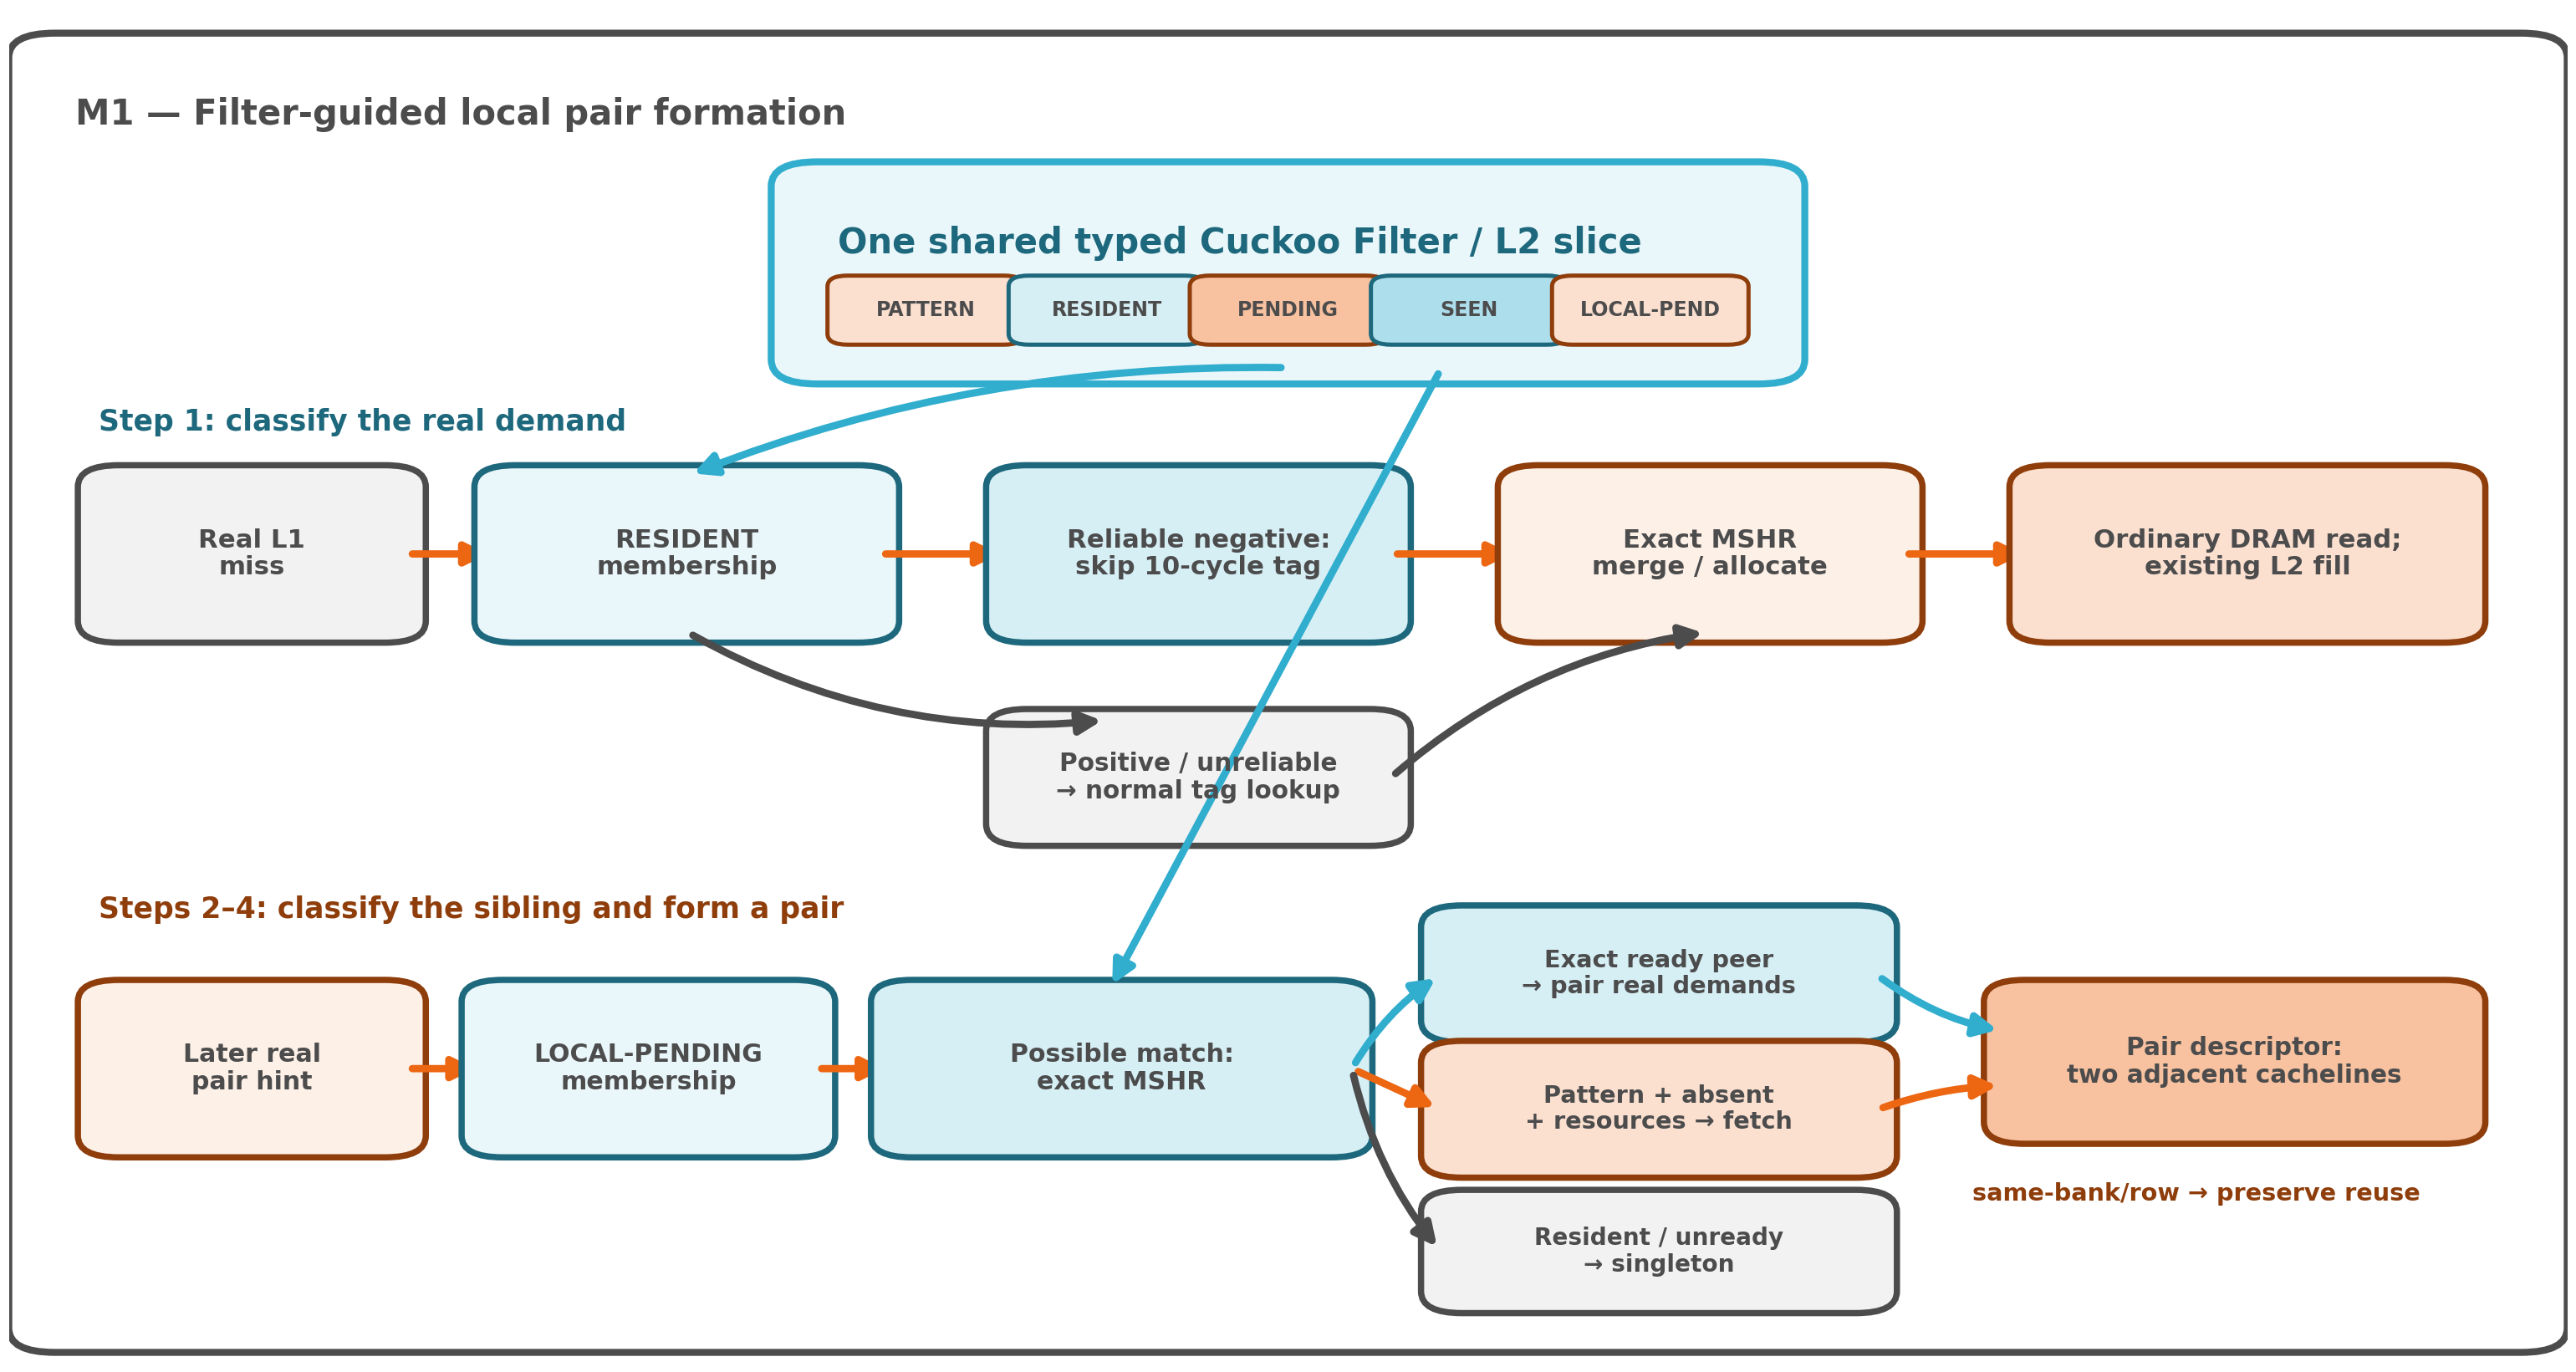
\includegraphics[width=\columnwidth]{Figure/M1.png}
  \caption{Local Pairing learns adjacent demand pairs, removes a line that is already
  resident or covered by an in-flight read, and otherwise fetches the pair
  with one HBM read.}
  \label{fig:cupath-m1}
\end{figure}

\subsection{Cuckoo-Filter-Guided Remote Aggregation}
\label{sec:design-m2}

Motivated by O4 and O5, Remote Aggregation combines remote requests before they consume
wafer-network work. Private L1 MSHRs cannot observe duplicate misses from
different L1 caches, while owner-L2 MSHRs act only after the requests have
crossed the wafer. Requester RDMA is the first point that observes all remote
misses from one GPM. Remote Aggregation uses the typed Cuckoo Filter at this point to identify
which requests may share existing work before consulting the exact RDMA state.
The Filter does not replace the request table or form packets by itself. It
guides both exact-line coalescing and the discovery of an active owner-page
batch, and prevents unnecessary lines from entering that batch.

For every issued remote line, Remote Aggregation inserts a \textsc{Remote-Pending} fingerprint
into the Filter. The exact requester-RDMA request table retains the complete
transaction, including its process, owner GPM, cacheline, write epoch, and
bounded waiter list. When another remote read arrives, Remote Aggregation first queries
\textsc{Remote-Pending}.

A reliable negative Filter result shows that no represented transaction is
outstanding for the line. Remote Aggregation therefore skips the exact same-line lookup,
allocates a new request-table entry, and inserts \textsc{Remote-Pending}. A
possible Filter match instead triggers an exact request-table lookup. If the
transaction exists, Remote Aggregation adds the demand to its waiter list, allowing one remote
operation to serve all matching L1 misses. A false positive simply allocates a
new entry and proceeds as a negative result.

A newly allocated line becomes the leader of a remote transaction. Remote Aggregation forms a
batch key from the process, owner GPM, and 4-KB page and queries
\textsc{Remote-Batch} before accessing the exact batch table.

A reliable negative Filter result shows that no joinable batch is represented
for the key. Remote Aggregation allocates a batch descriptor, records the leader in its bitmap,
and inserts \textsc{Remote-Batch}. A possible Filter match triggers an exact
batch-table lookup. The new leader joins a matching descriptor when a bitmap
position remains available. A false or stale match, or a full descriptor,
causes Remote Aggregation to allocate a new batch without delaying the request.

A batch remains represented by \textsc{Remote-Batch} only while at least one
matching descriptor can accept another line. When the last joinable descriptor
becomes full or is selected for egress, Remote Aggregation removes that state. A singleton is
sent as an ordinary remote read, while multiple leaders in one bitmap cross
the network as one packet. Owner RDMA expands the bitmap into ordinary
cacheline accesses to the existing owner L2. Returned lines are matched to
their exact request-table entries and fanned out to every waiting L1 request.
Remote Aggregation never delays a request to wait for a future partner and uses no batching
timeout.

The Filter also controls whether a predicted page-local line may use a free
position in an existing batch. \textsc{Pattern} must indicate a relation
trained by real remote demands, while reliable negative results for
\textsc{Resident} and \textsc{Remote-Pending} show that the line is neither
cached locally nor already in flight. \textsc{Remote-Batch} must also indicate
that a compatible batch may exist. Possible matches are confirmed using the
corresponding exact L2, request-table, predictor, and batch-table state. Remote Aggregation
admits the line only when the exact batch belongs to the same owner and page
and still has a free bitmap position. Otherwise, the candidate is discarded
without creating a packet or delaying a demand.

When the response completes, Remote Aggregation fans out the data, releases the exact request
entry, and deletes its \textsc{Remote-Pending} fingerprint. If a Filter result
or update is unavailable, Remote Aggregation uses the conservative exact path. Writes advance
the transaction epoch so that a read cannot merge with stale state. The Filter
therefore removes avoidable line-table and batch-table lookups, locates
possible aggregation opportunities, and filters predicted candidates. The
exact request table and bitmap batch remain authoritative.

\begin{figure}[t]
  \centering
  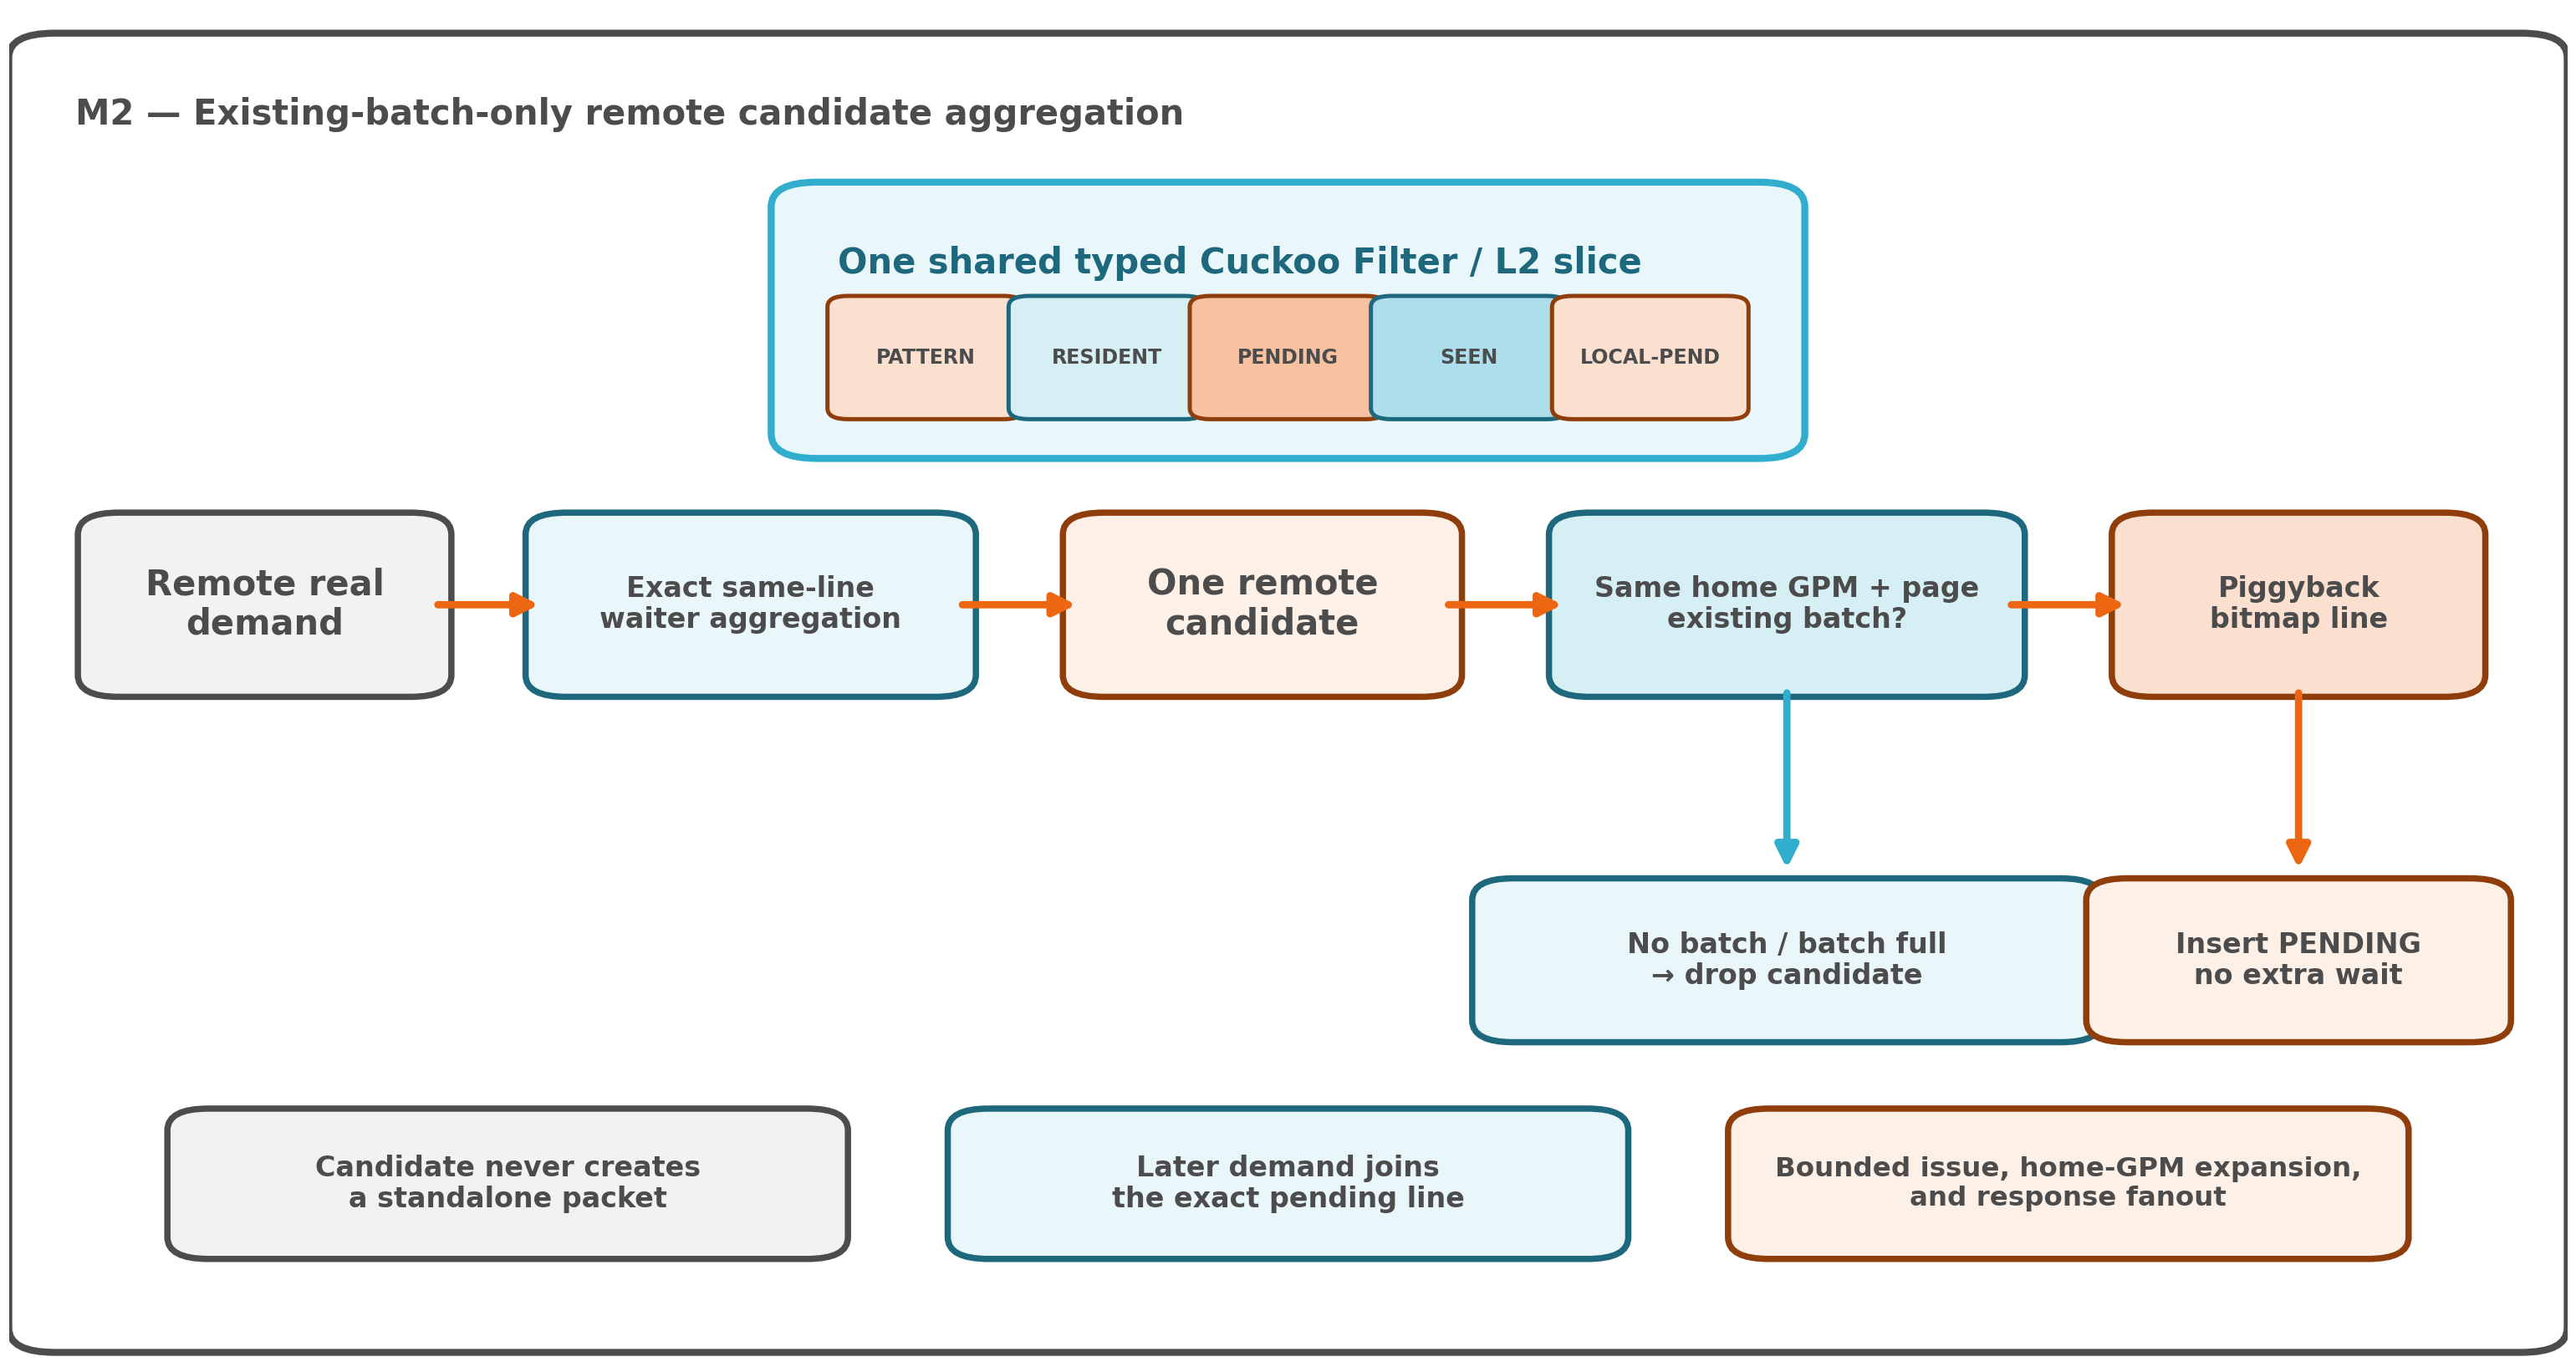
\includegraphics[width=\columnwidth]{Figure/M2.png}
  \caption{The typed Cuckoo Filter identifies possible in-flight duplicates,
  locates a joinable owner-page batch, and filters predicted candidates. Exact
  RDMA tables confirm matches before identical lines are merged or different
  lines are grouped into one packet.}
  \label{fig:cupath-m2}
\end{figure}

\subsection{Cuckoo-Filter-Guided Remote Reuse}
\label{sec:design-m3}

Motivated by O6, Remote Reuse uses the existing requester L2 to retain remote data only
after real accesses reveal reuse. The baseline sends a remote return directly
to requester L1. Once the line leaves L1, a later access repeats requester
RDMA, wafer-network, owner-L2, and possibly owner-HBM work. Filling every
remote return into requester L2 would avoid some traversals but would also
consume capacity for lines that never recur. Remote Reuse uses \textsc{Seen} to
distinguish recurring lines from one-time remote data and adds no new cache
level.

After requester RDMA finds no matching in-flight transaction, Remote Reuse checks
\textsc{Resident} and \textsc{Seen} before issuing the remote request.

Reliable negative results for both types identify a cold remote line that is
neither represented as resident nor previously observed. Remote Reuse bypasses the
otherwise guaranteed-miss requester-L2 tag lookup and sends the request to the
owner GPM. The first completed access returns to L1 without filling requester
L2 and inserts \textsc{Seen}. A possible Filter match indicates that the line
may be retained or recurring and triggers an exact requester-L2 tag lookup.
An L2 hit completes locally, while an exact miss follows the remote path and
preserves the reuse evidence for the returning response.

A response with real recurrence evidence becomes eligible for a clean fill in
requester L2. The second completed access supplies such evidence, and multiple
real demands merged by Remote Aggregation can establish it within one remote transaction. A
predicted line qualifies only if a real demand claims it while the transaction
is in flight. A successful fill updates \textsc{Resident}, allowing a later
access to complete locally without another wafer traversal.

Every fill remains best effort. Remote Reuse may use an invalid way or replace another
clean remote line, but it does not evict ordinary local data. A dirty, locked,
active-MSHR, or stale-generation victim rejects the fill. An unclaimed
predicted return can use only an invalid way. If a fill fails, \textsc{Seen}
remains recorded so that a later real access can try again. Remote writes
invalidate the corresponding reuse history and advance the exact transaction
epoch.

\begin{figure}[t]
  \centering
  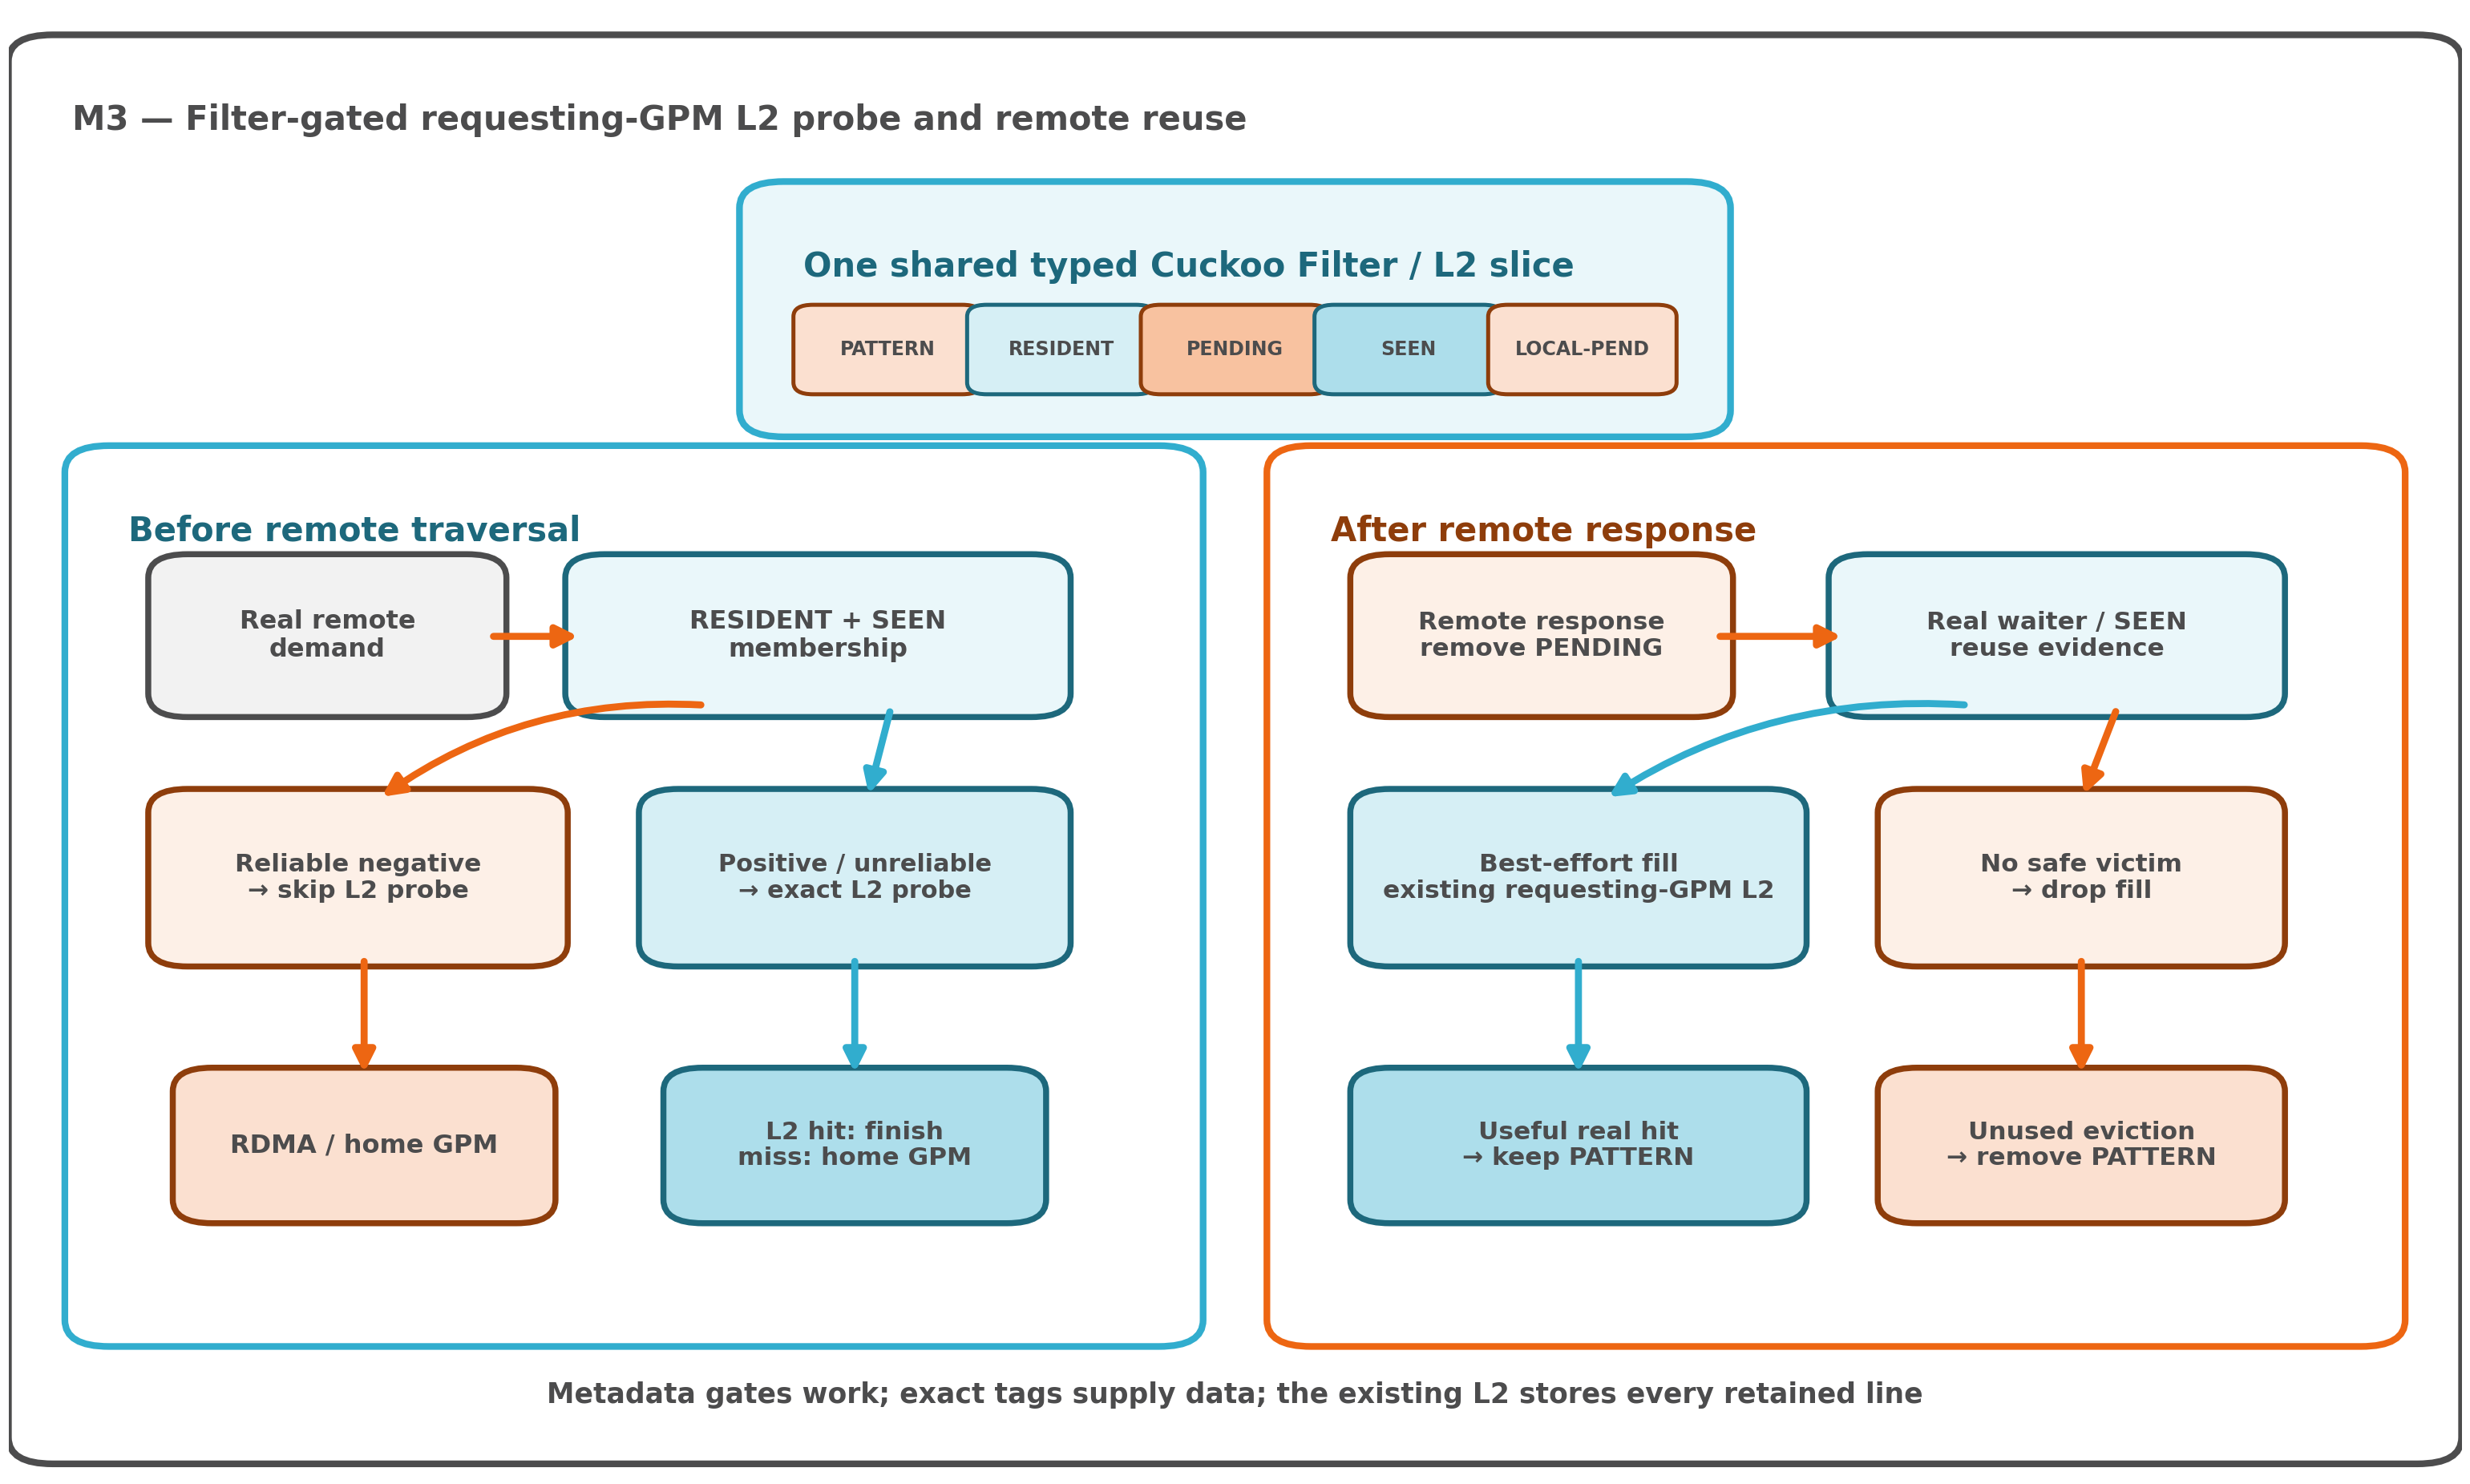
\includegraphics[width=\columnwidth]{Figure/M3.png}
  \caption{Remote Reuse bypasses known-miss requester-L2 lookups and retains a remote
  return in the existing requester L2 only after real accesses reveal reuse.}
  \label{fig:cupath-m3}
\end{figure}

\subsection{End-to-End Composition}

The three transformations operate on one request lifecycle. Local Pairing uses local demand
history and L2 residency to choose the amount of HBM work. Remote Aggregation uses global
request visibility and \textsc{Remote-Batch} state at requester RDMA to remove
duplicates and locate compatible network work. Remote Reuse uses completed remote
activity to decide whether another wafer traversal can be avoided. The typed
Cuckoo Filter carries compact lifecycle state between these decisions, while
exact structures preserve correctness. No mechanism waits for a speculative
opportunity. When evidence, metadata bandwidth, or downstream capacity is
unavailable, CuPath continues along the baseline path.


% !TeX root = ../main.tex
\section{Evaluation Methodology}
\label{sec:evaluation}

\subsection{Simulation}

\textbf{Simulation.}
We extend MGPUSim~\cite{sun2019mgpusim} with distributed page placement, a
packet-switched mesh, RDMA endpoints, detailed cache and HBM timing, and the
instrumentation required to model the complete memory path of a wafer-scale
GPU.  We model 48 GPMs connected by a $7\times7$ mesh, with the remaining tile
hosting the central I/O and control components.  Each link provides 768~GB/s
of bandwidth and incurs 32 cycles of switch latency, consistent with prior
multi-chip and wafer-scale studies
\cite{arunkumar2017mcm,feng2024barre}.  Each GPM represents one quarter of an
AMD MI100-class GPU.  Four GPMs collectively provide the compute, cache,
memory capacity, and memory bandwidth of one MI100
\cite{techpowerup_mi100}.  This scaling keeps cycle-level simulation of the
48 GPM system tractable while preserving its aggregate resource ratios.

\textbf{Cache and memory hierarchy.}
Each GPM contains 32 CUs organized as eight shader arrays.  Every CU has a
private 16~KB, four-way L1 vector cache with a 10-cycle access, 16 MSHRs, and
at most 160 concurrent transactions.  Each shader array also has a 16~KB
scalar cache and a 32~KB instruction cache.  The GPM-wide 4~MB L2 is divided
into four independently accessed 1~MB partitions.  Each partition is 16-way
associative, accepts 16 requests per cycle, contains 64 MSHRs, and charges a
10-cycle directory lookup to both
hits and misses.  Four memory controllers connect the L2 to 8~GB of local HBM
with 1.23~TB/s aggregate bandwidth.  Each RDMA endpoint processes eight
transfers per cycle, charges 10 cycles for an endpoint traversal, and tracks
up to 64 requester and 64 owner transactions.  Table~\ref{table:BaselineConfig}
summarizes the modeled system.

\textbf{CuPath modeling.}
The MCM-GPU design introduces a GPM-side, remote-only L1.5 cache between L1
and L2 and explores reallocating L2 capacity to that new level
\cite{arunkumar2017mcm}.  CuPath does not add an L1.5 cache, a victim cache,
or another independently addressable cache.  Baseline and CuPath therefore
use identical L1 and L2 capacities, associativities, ports, MSHRs, and lookup
latencies.  CuPath adds one metadata-only Cuckoo Filter and a bounded 16-line
M1 response buffer per L2 partition, together with bounded local and remote
prediction state.  The response buffer holds an adjacent line returned by a
paired HBM access until a matching demand consumes it or replacement removes
it.  A retained remote response is instead inserted as a clean line through
the existing L2 fill and replacement path.  Exact cache tags, MSHRs, and RDMA
transaction tables remain authoritative.  All
configurations also use the same TLBs and 4~KB physical page mapping, so every
reported difference comes from cache, HBM, RDMA, and network processing below
address translation.

\textbf{Execution scope.}
Each experiment continues until 78{,}600 workgroups have completed across the
48-GPM system.  This represents approximately 51 completed workgroups for each
of the wafer's 1,536 CUs and is sufficient to capture steady execution beyond
the initial transient \cite{baruah2020griffin}.  We terminate at a workgroup
boundary because prior studies show that workgroup completion rates stabilize
after warmup \cite{avalos2021principal,liu2023photon}.  The threshold does not
change kernel launches, workgroup IDs, partitioning, or GPU assignment.  A
workload with fewer workgroups runs to completion, and all configurations use
the same termination rule.

\begin{table}[t]
  \centering
  \caption{Baseline wafer-scale GPU and CuPath configuration.}
  \label{table:BaselineConfig}
  \footnotesize
  \begin{tabularx}{\columnwidth}{@{}l>{\raggedright\arraybackslash}X@{}}
    \toprule
    \textbf{Module} & \textbf{Configuration} \\
    \midrule
    Wafer & 48 GPMs, 1.0~GHz, $7\times7$ mesh \\
    Compute & 32 CUs/GPM, eight shader arrays/GPM \\
    L1 vector & 16~KB/CU, 4-way, 10 cycles,
                16 MSHRs \\
    L1 scalar & 16~KB/shader array, 4-way, 16 MSHRs \\
    L1 instruction & 32~KB/shader array, 4-way, 16 MSHRs \\
    Shared L2 & 4~MB/GPM, four partitions, 16-way, 64 MSHRs/partition,
                16 req./cycle/partition, 10-cycle lookup \\
    HBM & 8~GB/GPM, four controllers, 1.23~TB/s, BL4 \\
    RDMA endpoint & 8 transfers/cycle, 10-cycle processing,
                    64 outstanding/direction \\
    Mesh link & 768~GB/s, 32-cycle switch latency, 16-B flit \\
    \midrule
    \multicolumn{2}{l}{\textit{CuPath additions}} \\
    Cache capacity & No L1.5 or new addressable cache; baseline L1/L2 unchanged \\
    Typed Filter & One shared array/L2 partition, 4K buckets, four slots/bucket,
                   13-bit fingerprint \\
    Filter ports & 1-cycle lookup/update, 16 lookups and 16 updates/cycle/partition \\
    M1 state & 64 observed regions and 16 returned lines/L2 partition \\
    Remote predictor & 256 entries/requesting GPM \\
    M1 & Filter-guided paired HBM access \\
    M2 & Up to eight lines/packet, 64 packet descriptors/requesting GPM \\
    M3 & No separate history; best-effort clean fill into existing L2 \\
    \bottomrule
  \end{tabularx}
\end{table}

\subsection{Ablation Configurations}

We run five configurations from the same frozen simulator binary.
\emph{Baseline} disables every CuPath transformation.  \emph{M1} enables the
complete local request-pairing path: reliable \textsc{Resident} negatives
bypass guaranteed-miss L2 tag lookups, and typed membership state admits at
most one predicted sibling into the triggering miss's paired HBM access.
\emph{M2} uses \textsc{Remote-Pending} to guide exact same-line
deduplication and \textsc{Remote-Batch} to locate joinable, work-conserving
home-GPM/page packets. Predicted remote candidates can use only a free position
in a Filter-identified and exactly confirmed existing batch;
requesting-GPM L2 reuse is off.  \emph{M3} enables \textsc{Seen}/
\textsc{Resident}-guided requesting-GPM L2 probe gating and reuse without remote
batching or candidate generation.  \emph{Complete} enables M1--M3.  Row-aware DRAM
reordering remains disabled in all five configurations.

In the complete configuration, the stages operate on the surviving request
population.  A requesting-GPM L2 termination never enters requesting-GPM RDMA, and a
coalesced RDMA waiter does not create a network or home-GPM memory request.  We therefore place
counters at each boundary and report both eliminated work and end-to-end
performance, rather than treating the three stage speedups as additive.

\subsection{Hardware Overhead}

We estimate CuPath's storage and area overhead with CACTI~7.0
\cite{balasubramonian2017cacti} at 32~nm.  Each L2 partition has a 4K-bucket
Typed Filter with four slots per bucket.  Each slot contains a 13-bit
fingerprint, three type bits, one valid bit, and a four-bit reference count,
requiring 42~KiB per Filter.  We model each Filter as 16 banks with two read
ports and one write port per bank.  In the conflict-free case, this organization
supports 16 two-bucket lookups and 16 updates per cycle.  The 256-entry remote
predictor is conservatively budgeted at 64~B per entry, or 16~KiB per GPM.
The four Filters and predictor therefore require 184~KiB per GPM, equal to
4.49\% of the 4-MiB L2 data capacity.

CACTI estimates 0.358~mm$^2$ for each Filter and 0.036~mm$^2$ for the remote
predictor.  The resulting CuPath area is 1.469~mm$^2$ per GPM.  A complete
4-MiB, 16-way L2, modeled as four 1-MiB partitions and including data arrays,
tag arrays, and peripheral circuitry, occupies 54.510~mm$^2$.  CuPath therefore
adds 2.70\% area relative to the modeled L2.  Filter and predictor accesses take
0.523~ns and 0.241~ns, respectively, and fit within the 1-ns cycle.  The estimate
includes the arrays and their modeled ports, but excludes hashing, fingerprint
comparators, arbitration, bank conflicts, and CuPath control logic.

\subsection{Workloads and Execution}

We evaluate CuPath with 14 benchmarks from Hetero-Mark
\cite{sun2016hetero}, AMD APP SDK~\cite{amd_opencl_guide},
SHOC~\cite{danalis2010scalable}, and DNNMark~\cite{dong2017dnnmark}.
The suite has also been used by prior multi-GPU studies
\cite{wang2025oasis,li2023idyll,li2021improving,feng2024barre} and spans
local and remote accesses with both streaming and repeated data use.
Table~\ref{table:Benchmark} reports these two workload properties, the
workgroups actually admitted and retired in the formal run and the workload
allocation footprint measured immediately after allocation from the
simulator's 4-KB page counters.  We derive the labels from the latest Baseline
run.  \textbf{Remote} and \textbf{Local} identify whether most memory requests
are served by a remote or local home GPM.  \textbf{Repeated} indicates that L1
and L2 cache hits together serve more than half of read accesses, whereas
\textbf{Streaming} indicates that most reads pass through both cache levels
and continue toward memory.  Baseline and Complete allocate the same number of
pages and complete the same number of workgroups for every workload.

We choose the largest hundreds-of-MB or GB-scale input that remains tractable
in cycle-level simulation, following prior multi-GPU and wafer-scale studies
\cite{baruah2020griffin,li2023trans,xu2025exploring}.  Every footprint exceeds
the capacity of a single GPM's private and shared caches, forcing requests to
exercise local HBM and, under distributed page placement, remote home-GPM paths.

The runner records every launch, partition, observed workgroup count, and a
hash of the global workgroup set.  We reject a comparison if these identities
differ across configurations.

\begin{table}[t]
  \centering
  \caption{Benchmarks, access location, data use, completed workgroups, and footprint.}
  \label{table:Benchmark}
  \scriptsize
  \setlength{\tabcolsep}{3pt}
  \begin{tabularx}{\columnwidth}{lccXr}
    \toprule
    \textbf{Benchmark} & \textbf{Access} & \textbf{Data use} &
    \textbf{Completed WGs} & \textbf{Footprint} \\
    \midrule
    AES  & Local  & Repeated  & 78,600 & 1,024~MiB \\
    BT   & Local  & Streaming & 78,600 & 1,024~MiB \\
    FWT  & Local  & Streaming & 78,600 & 1,024~MiB \\
    FFT  & Local  & Streaming & 78,600 & 1,024~MiB \\
    FIR  & Local  & Repeated  & 78,600 & 1,024~MiB \\
    FWS  & Local  & Repeated  & 78,600 & 1,024~MiB \\
    I2C  & Remote & Repeated  & 78,600 & 1,029~MiB \\
    KM   & Local  & Repeated  & 73,728 & 390~MiB \\
    MM   & Remote & Repeated  & 78,600 & 1,024~MiB \\
    MT   & Remote & Streaming & 32,400 & 1,013~MiB \\
    PR   & Remote & Repeated  & 78,600 & 1,024~MiB \\
    RELU & Local  & Streaming & 78,600 & 2,560~MiB \\
    SC   & Local  & Repeated  & 78,600 & 512~MiB \\
    SPMV & Local  & Streaming & 78,600 & 1,081~MiB \\
    \bottomrule
  \end{tabularx}
\end{table}


\section{Results}
\label{sec:results}

\subsection{Overall Performance}

Figure~\ref{fig:cupath-performance} compares CuPath with Baseline using the
formal 14-workload campaign.  Every pair uses the same frozen binary,
benchmark input, architectural parameters, workgroup-completion rule, and
completed workgroup count; only the CuPath mechanisms differ.  CuPath achieves
a 1.465$\times$ geometric-mean speedup and improves 13 of the 14 workloads.
MM, FWS, and KM obtain the largest gains at 6.171$\times$,
4.155$\times$, and 2.511$\times$, respectively.  BT and FWT improve by
1.491$\times$ and 1.578$\times$, while I2C and RELU improve by
1.214$\times$ and 1.117$\times$.  The remaining workloads stay close to
Baseline, with SPMV at 0.999$\times$.  The result shows that CuPath provides
large gains when requests expose eliminable or aggregatable work, while its
work-conserving fallback keeps workloads with few opportunities near
Baseline.

\begin{figure}[t]
  \centering
  \includegraphics[width=\columnwidth]{../../akkalat/results/2026-07-22-baseline-complete-observation/cupath_baseline_complete_speedup.png}
  \caption{Normalized performance of CuPath relative to Baseline.  Baseline
  is normalized to 1.0 for every workload, and GM is the geometric mean across
  all 14 workloads.}
  \label{fig:cupath-performance}
\end{figure}

\subsection{Removing Work Along the Path}

Figure~\ref{fig:cupath-work} explains the speedup in terms of work that no
longer reaches a downstream component.  Weighted across the fourteen
workloads, Complete removes 22.6\% of L2 tag lookups, 4.6\% of unique remote
reads, 48.2\% of wire packets, and 30.8\% of repeated wafer traversals.  The
different columns peak on different applications: L2 filtering is strongest
for SPMV and MT, packet aggregation for AES, RELU, and KMeans, and requesting-GPM
L2 reuse for MM, FIR, SC, and I2C.  This separation supports the path-oriented
design: no single boundary exposes all four reductions.

CuPath does not obtain these gains by increasing aggregate memory traffic.
Complete reduces physical DRAM reads from 39.25 to 38.71 million (1.38\%) and
writes from 20.83 to 20.68 million (0.71\%).  The sample-weighted local
L2-miss-to-DRAM-issue latency falls from 38.12~ns in Baseline to 20.34~ns over
the ordinary and Filter-negative Complete issue populations.  We report these
populations separately in the machine-readable results; the comparison is not
an assumption that every miss takes the fast path.

\begin{figure}[t]
  \centering
  \includegraphics[width=\columnwidth]{../../akkalat/results/2026-07-17-filter-prefetch-v5-formal14/cupath_work_reduction.png}
  \caption{Percentage of baseline work removed at successive boundaries.
  The bottom row is weighted by the corresponding baseline work count.}
  \label{fig:cupath-work}
\end{figure}

\subsection{M1: Cuckoo-Filter-Guided Local Pairing}

M1 is a supporting transformation rather than the dominant source of
speedup.  It issues 261,615 local candidates over the full suite: 252,850
reach the DRAM-issue point and 8,765 lose a race to an ordinary demand;
176,447 are eventually useful.  Although these issued candidates are
additional logical accesses, exact MSHR merging and demand timing leave total
physical reads 0.35\% lower than Baseline and increase L2 MSHR-full cycles by
only 0.22\%.  FIR is the exception: M1 alone is 0.898$\times$ and increases
physical reads and writes, so we do not claim that local prediction is
universally beneficial.

The coupling experiment isolates why the Filter is still useful for mostly
local workloads.  Filter-only definite-miss elimination provides
1.0145$\times$ geometric mean, while ungated prediction provides only
1.0059$\times$.  Coupling the same predictor to \textsc{Pattern},
\textsc{Resident}, and \textsc{Pending} reaches 1.0188$\times$.  It removes
34.7\% of issued candidates while retaining 96.7\% of useful candidates,
raising useful-per-issued accuracy from 24.0\% to 35.5\%.  Additional DRAM
reads fall from 6,206 to 5,578 and demand-delay exposure events from 145,466
to 33,066.  Predictor-only records candidates but is exactly 1.0000$\times$,
confirming that observation itself is not counted as timing benefit.

Replacing Cuckoo membership with exact metadata changes the same screen only
from 1.0188$\times$ to 1.0192$\times$.  The Cuckoo design observes four false
positives in 273,146 queries (0.0015\%).  Thus the Filter does not move data or
create prediction benefit by itself; it compactly rejects avoidable work and
tracks the request lifecycle with little loss relative to exact metadata.

\subsection{M2: Cuckoo-Filter-Guided Remote Aggregation}

M2 is the largest standalone contributor.  Complete records 4.24 million
real demands merged by exact RDMA line state and 2.52 million predicted lines
piggybacked into existing home-GPM/page packets.  Because a real demand can take
over a candidate before batch insertion, the aggregate counters do not expose
the intersection of these two populations; we therefore do not relabel every
useful prediction as an avoided packet.  The exact merge and wire-packet
counters independently establish the reductions.

\subsection{M3: Cuckoo-Filter-Guided Remote Reuse}

M3 bypasses 23.41 million exact requesting-GPM L2 probes when \textsc{Resident}
and \textsc{Seen} reliably prove absence, 42.6\% of eligible unique-request
probe opportunities.  The remaining probes produce 27.23 million physical
L2 hits and satisfy 28.21 million logical responses through exact waiter
fanout.  M3 installs 7.06 million remote-clean lines in the existing L2;
0.996 million are observed to retire unused, a 14.1\% lower bound because
lines still resident at termination are unclassified.  Invalid ways absorb
5.35 million fills and older remote-clean lines absorb the remaining 1.71
million; no ordinary local-clean line is displaced.  The largest
workload-level sum of per-slice peaks occupies 37.5\% of wafer L2 lines, a
conservative non-simultaneous upper bound rather than an average footprint.
Of the unused retirements, 160,257 carry candidate provenance and remove the
associated \textsc{Pattern}.  A useful patterned hit instead keeps
\textsc{Pattern} eligible; the aggregate counter does not isolate that subset
from all requesting-GPM L2 hits.

\subsection{Sensitivity and Limitations}

Figure~\ref{fig:cupath-sensitivity} varies only the parameters needed to audit
the selected point.  Across four workloads, all tested points span
1.2713$\times$--1.2817$\times$, compared with 1.2757$\times$ for the
32K-slot, 13-bit, 64-entry, one-cycle point.  Reducing the Filter to 16K slots
raises insertion failures from 27 to 156,726, whereas 64K slots, 16
fingerprint bits, or a 256-entry predictor changes geometric mean by less
than 0.5\%.  A zero-cycle lookup reaches 1.2791$\times$, only 0.27\% above the
selected point; the result therefore does not depend on a free Filter lookup.

The long runs expose a limitation hidden by the short screen.  Across the
fourteen Complete runs, correctness-critical \textsc{Resident} and
\textsc{Pending} have zero insertion failures, but capacity pressure causes
9.42 million \textsc{Pattern} and 5.81 million \textsc{Seen} attempts to fail
closed.  These failures suppress optional prediction or reuse and cannot
change demand correctness, but they bound coverage.  The modest
1.187$\times$ Remote-group speedup and M1's FIR regression likewise show that
CuPath is constrained by available aggregation and safe idle opportunities,
not by an unlimited speculative upper bound.

A controlled simulator-runtime screen uses seven representative workloads,
all five configurations, 192 drained workgroups, one host worker, and the
same binary.  Normalized by simulated GPU time, Complete costs
1.190$\times$ Baseline; this is simulator overhead, not hardware performance.

\begin{figure}[t]
  \centering
  \includegraphics[width=\columnwidth]{../../akkalat/results/2026-07-17-filter-prefetch-v5-sensitivity/cupath_sensitivity.png}
  \caption{Four-workload sensitivity.  Orange marks the selected point and
  blue marks alternatives; all use the same frozen binary.}
  \label{fig:cupath-sensitivity}
\end{figure}


\bibliographystyle{IEEEtranS}
\bibliography{refs}

\end{document}
